\documentclass[12pt,openbib]{report}
\usepackage[utf8]{inputenc}
\usepackage[russian]{babel}

\emergencystretch=25pt

\usepackage{amsmath, amsfonts, amssymb, latexsym, graphicx, amsmath, geometry, indentfirst, longtable, array}

\usepackage[unicode]{hyperref}
\usepackage{pdfpages}


\graphicspath{{images/}{pic/}}

\makeindex

\pagestyle{empty}

\renewcommand{\baselinestretch}{1.3}

\geometry{verbose,a4paper,tmargin=2.0cm,bmargin=2.0cm,lmargin=2.5cm,rmargin=1.0cm}


\newcounter{pic}
\renewcommand{\thepic}{\arabic{pic}}
\newcommand{\pic}{\par\refstepcounter{pic}
\vspace{5mm} \centerline{Рис.\,\arabic{pic}}}

\newtheorem{opr}{\hspace{5mm} Определение}[chapter]
\newtheorem{teo}{\hspace{5mm} Теорема}[chapter]
\newtheorem{pri}{\hspace{5mm} Пример}[chapter]
\newtheorem{pre}{\hspace{5mm} Предложение}[chapter]
\newtheorem{utv}{\hspace{5mm} Утверждение}[chapter]
\newtheorem{zam}{\hspace{5mm} Замечание}[chapter]
\newtheorem{lem}{\hspace{5mm} Лемма}[chapter]
\newtheorem{sle}{\hspace{5mm} Следствие}[chapter]


\renewcommand{\theequation}{\arabic{chapter}.\arabic{section}.\arabic{equation}}


\begin{document}
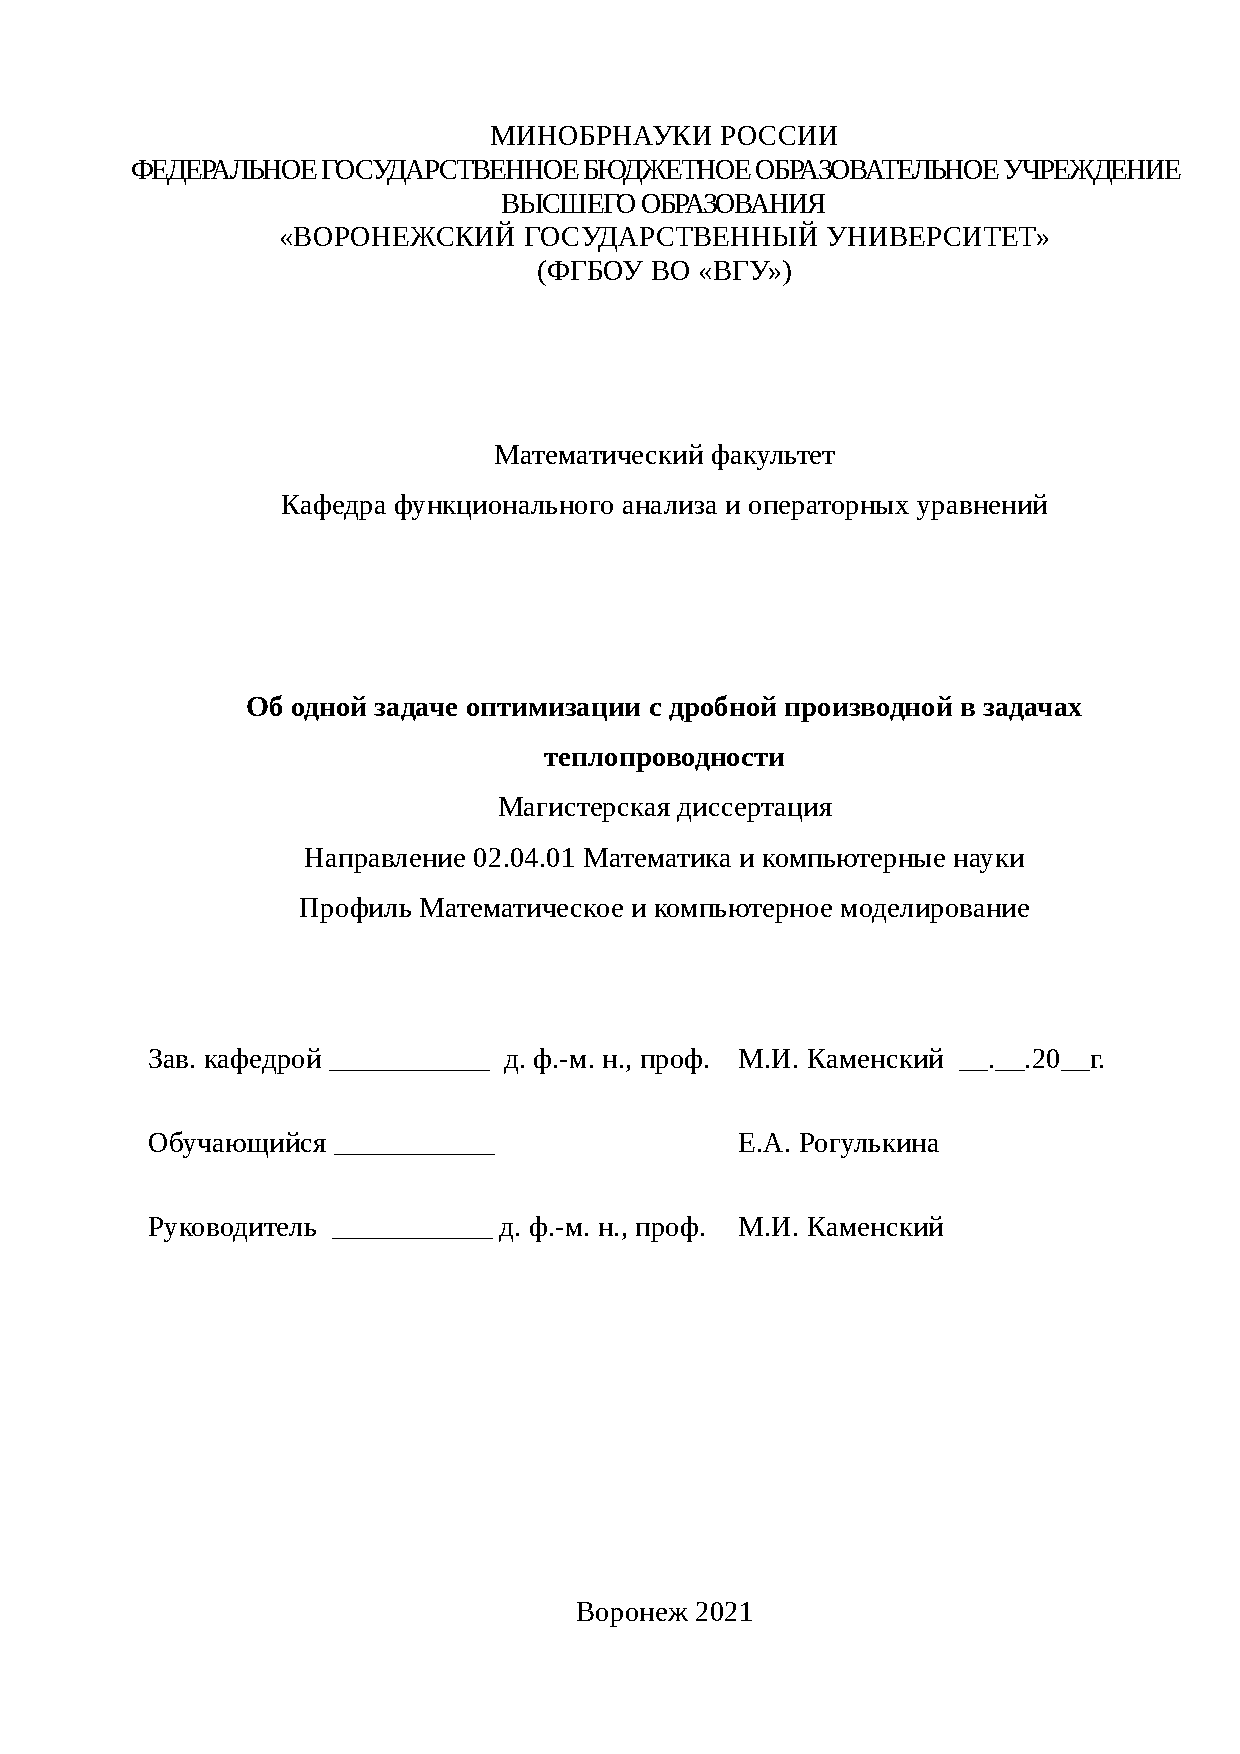
\includepdf{titlepage.pdf}
\Large
\tableofcontents
\newpage

\begin{center}
\section*{Введение}
\addcontentsline{toc}{section}{Введение}
\end{center}
Анализ истории экономики показывает, что в спокойные периоды состояния общества преобладают методы, носящие равномерный характер,
тогда как в более беспокойные периоды предпочтение отдается динамическим подходам, требующим новых математических методов и понятий.
Например, как отмечается в \cite{kozyreva}, при оценке стоимости нематериальных активов (НМА) интеллектуальной собственности (ИС)
мы имеем дело с фундаментальным противоречием между принципом бухгалтерского учета и свойствами экономики знаний (или алгебраическими свойствами самих знаний).
Бухгалтерия основана на принципах обычной арифметики: если где"=то, что-то прибавилось, должно убыть в другом месте.
Однако, как замечено, знания подчиняются совсем другим алгебраическим правилам.
На это обстоятельство обращали внимание и нобелевские лауреаты Л.~Канторович и В.В.~Леонтьев. Это приводит к поиску новых подходов и математических понятий.
Так, Эдвардсон \cite{kozyreva} предлагает стоимости интеллектуального капитала не складывать, а умножать. В русле этих исследований академиком
РАН В.П. Масловым предлагается <<квантовая экономика>> с использованием <<нелинейной арифметики>>.
Настоящая квалификационная работа посвящена применению нелинейного осреднения В.П. Маслова и решению некоторых задач оптимизации в экономических процессах.

В первой главе рассматриваются неоклассические производственные функции.

Во второй главе приводится производственная функция\linebreak
В.П.~Маслова и задачи оптимизации производства.


\chapter{Неоклассические прозводственные функции}

\section{Понятие производственной функции}

{\it Производственная функция} одной независимой переменной $x$
\begin{equation}\label{f11}
y=f(x)
\end{equation}
---это функция, у которой $x$ принимает значения
объемов {\it затрагиваемого} или {\it используемого ресурса}
(фактора производства), а $y$--- значения объемов {\it выпускаемой
продукции}

В связи с этим, такая производственная функция $f$ называется {\it
одноресурсной} или {\it однофакторной} ПФ, ее область определения---
множество неотрицательных действительных чисел (т.е. $x\ge0$, $x\in
\mathbb{R}^+$).

Запись $y=f(x)$ означает, что если ресурс затрагивается в количестве
$x$ единиц, то продукция выпускается в количестве $y=f(x)$. Символ
$f$--- является характеристикой {\it производственной системы,}
преобразующей ресурс в выпуск.

Как отмечено в \cite{MaslovAksiom}, c. 157, в макроэкономической теории принято
считать, что $y$--- это {\it максимально} возможный объем выпуска
продукции при затраченном ресурсе $x$ единиц. Однако в
макроэкономике, такое понимание не совсем корректно, так как
возможно, при другом распределении ресурсов между другими
структурными единицами экономики выпуск мог бы быть и большим.

Поэтому, в этом случае, ПФ характеризует статически устойчивую связь
между затратами ресурсов, а более общей является символика
$y=f(x,a)$, где $a$--- вектор параметров ПФ.

Типичным представлением широкого класса однофакторных ПФ является
степенная функция
\begin{equation}\label{f12}
y=f(x)=ax^\beta,
\end{equation}
где $a>0$, $x\ge0$,$0<\beta<1$.

Очевидно. что эта функция обладает следующими свойствами
$$f(x)\ge0,\hspace{10mm}\frac{df}{dx}>0,\hspace{10mm}\frac{d^2}{dx^2}<0,$$
из которых следует, что с ростом величины затраченного ресурса $x$
растет и объем выпуска $y$, однако, при этом, каждая дополнительная
единица ресурса дает все меньший прирост объема у выпускаемой
продукции.

Это обстоятельство отражает фундаментальное положение {\it
экономической теории}, называемое {\it законом убывающей
эффективности}.

Каковы единицы измерения выпуска и затрат? Если, к примеру, взять
затраты труда, то кажется естественным измерять их временем,
затраченным на изготовление продукции. Однако при изготовлении
продукции, используется обычно труд разного рода, разной
квалификации и т.д. То есть, затраты труда неоднородны, а
соизмерение неоднородных видов труда, пока остается нерешенной
проблемой в экономической теории.

Не вникая далее в эту проблему, будем предполагать, что применяемый
при изготовлении продукции труд однороден и однородны отдельные
единицы затрачиваемого капитала. Также будем считать, что на
микроэкономическом уровне, затраты и выпуск измеряются как в {\it
натуральных}, так и в {\it стоимостных} единицах. На
макроэкономическом уровне, затраты и выпуск измеряются, как правило,
в стоимостных показателях.

Формально ПФ записывается следующим образом:
\begin{equation}\label{f13}
Y=(x_1,\dots,x_n),
\end{equation}
где $Y$ -- объем выпуска, $x_i$ -- объем $i$ -- го ресурса.
Предполагается, что функция $F$ удовлетворяет некоторым условиям,
вытекающим из общеэкономических соображений. Вид функции и некоторые
ограничения на значения параметров вытекают, как правило, из
теоретических представлений о структуре и функционирования
моделируемого объекта, а конкретные численные значения параметров
находятся в результате обработки, имеющейся в распоряжении
исследователя информации. Это могут быть временные ряды показателей
ресурсов и выпуска, результаты пространственных или
пространственно--временных выборок, данные о технико-экономических
характеристиках, используемых, потенциально доступных или
проектируемых технологий, агрегатов, производственных комплексов.
Параметры оценивают в основном методами регрессивного анализа.
Полученные таким образом ПФ представляют собой статистические
зависимости между ресурсами и выпуском. В работах западных
экономистов неоклассического направления значения параметров ПФ
часто определяют исходя из гипотезы о равенстве отношения предельных
производительностей ресурсов отношению цен на них (в качестве <<цены
труда>>, рассматривают среднюю ставку заработной платы, а <<цены
капитала>> --- норму процента), или о равенстве эластичностей
выпуска по ресурсам и долей их владельцев в доходе.

Иногда ПФ записывают в более общем, чем (\ref{f13}) виде:
\begin{equation}\label{f14}
G(Y,x_1,\dots,x_n)=0.
\end{equation}

Выражение (\ref{f14}) называют также {\it уравнением производственной
поверхности}. Его можно обобщить на случай совместного производства
нескольких видов продукции:
\begin{equation}\label{f15}
G(Y_1,\dots,Y_m,x_1,\dots,x_n)=0.
\end{equation}

Но такие многопродуктивные производственные поверхности встречаются
лишь в сугубо теоретических работах.

Общепринятого мнения, каким набором свойств, вытекающих из
общеэкономических соображений, должна обладать ПФ вида (\ref{f13}), не
существует. Однако, обычно требуется, чтобы она обладала всеми или
хотя бы некоторыми из следующих свойств:

1) $F(0,\dots,0)=0$, т.е. выпуск невозможен при отсутствии ресурсов;

2) Если $x'_i>x_i$, $i=1,\dots,n$, то
$F(x_1,\dots,x_n')>F(x_1,\dots,x_n)$, т.е. при увеличении затрат
всех ресурсов выпуск растет;

3) $\frac{\partial F}{\partial x_i}\ge0$, $i=1,\dots,n$, т.е. с
увеличением затрат любого из ресурсов, при неизменном количестве
остальных, выпуск не уменьшается.

4) $\frac{\partial^2 F}{\partial x_i^2}\le0$, $i=1,\dots,n$, т.е. с
увеличением затрат любого из ресурсов, при неизменном количестве
остальных, эффективность вовлечения в производство дополнительной
его единицы не возрастает (принцип убывающей отдачи последовательных
вложений);

5) $\frac{\partial^2 F}{\partial x_i\partial x_j}\le0$,
$i=1,\dots,n$, $j=1,\dots,n$, т.е. эффективность затрат любого из
ресурсов, при увеличении затрат какого-либо другого ресурса и
неизменном количестве остальных, не снижается;

6) $F(x_1,\dots,x_n)$ строго квазиуизогнута;

7) $F(x_1,\dots,x_n)$ вогнута (выпукла вверх)

Это более жесткая формулировка принципа убывающей отдачи
последовательных вложений, из которой, в частности, следует свойство
4;

8) $F(x_1,\dots,x_n)$ однородна степени $\lambda$, т.е.
$F(ax_1,\dots,ax_n)=a^\lambda F(x_1,\dots,x_n)$. При $\lambda>1$ с
увеличением масштабов производства его эффективность растет
(растущая отдача или экономия масштаба), при $\lambda<1$--- падает
(падающая отдача или потери от масштаба), при $\lambda=1$--- не
меняется. В одних случаях значение $\lambda$ оценивается статически,
в других на него накладываются априорные ограничения. Так, в
подавляющем большинстве малоразмерных моделей экономического роста
предполагается, что $\lambda=1$.

Однако не все ПФ и не при всех значениях входящих в них переменных
обладают перечисленными свойствами. Иногда (хотя и достаточно редко)
применяют ПФ, для которых не выполняются даже первых три свойства,
хотя они наиболее естественны. Часто требуется, чтобы ПФ обладала
указанными свойствами не при всех, а лишь при <<экономически
осмысленных>> или реально достижимых значениях переменных. Множество
таких значений называют {\it экономической областью}.

Иногда требуется, чтобы ПФ помимо указанных выше свойств обладала и
некоторыми другими. Так, довольно часто налагаются ограничения на
значения ПФ или ее первых производных при стремлении одного из
аргументов к нулю или бесконечности (т.н. асимптотические условия).
Наиболее простое (и естественное для случая двухфакторной
макроэкономической ПФ) из них состоит в том, что значение функции
равно нулю при нулевом значении любого из аргументов.

Однородную ПФ произвольной степени, имеющую положительные первые
частные производные, отрицательные вторые частные производные и
положительные смешанные частные производные по всем факторам
производства, часто называют {\it неоклассической}.

ПФ позволяет рассчитать ряд важных характеристик, описывающих
различные стороны исследуемой производственной единицы. Наиболее
часто рассчитывают следующие характеристики:

1) предельная производительность (предельный продукт) $i$-- го
фактора, $\frac{\partial Y}{\partial x_i}$. Показывает, насколько
увеличится выпуск при увеличении затрат $i$-- го фактора на одну
(малую) единицу, при неизменном количестве остальных факторов.
Обычно предельная производительность $\frac{\partial Y}{\partial
x_i}$ меньше средней $\frac{ Y}{ x_i}$.

2) Частная эластичность выпуска по $i$-- му фактору (частная
факторная эластичность), $\frac{\partial Y}{\partial
x_i}\cdot\frac{x_i}Y$. Показывает, на сколько процентов увеличится
выпуск при увеличении затрат $i$-- го фактора на 1\% при неизменном
количестве остальных факторов. представляет собой отношение
предельной производительности к средней.

3) Эластичность производства
$$\pi(x_1,\dots,x_n)=\lim_{\lambda\to1}\frac\lambda{F(\lambda
x_1,\dots,\lambda x_n)}\cdot\frac{\partial F(\lambda
x_1,\dots,\lambda x_n)}{\partial\lambda}.$$

Показывает, на сколько процентов увеличится выпуск при увеличении на
$1\%$ затрат каждого фактора является локальной характеристикой
эффекта масштаба.

Очевидно, что $$\pi(x_1,\dots,x_n)=\sum_i\frac{\partial Y}{\partial
x_i}\cdot\frac{x_i}Y.$$

4) Предельная норма замены (замещения) $i$-- го фактора $j$-- м.
Показывает количество $j$-- фактора, которое требуется для замены
единицы $i$-- го фактора при сохранении на неизменном уровне объема
выпуска и количества остальных факторов. Обозначается обычно
$R_{ji}$ и, по определению, равна: $$R_{ji}=-\frac{\partial
x_j}{\partial x_i},\mbox{ при }Y=const,\,x_k=const,\,k\neq i,j.$$
Очевидно, что $R_{ij}=\frac{\partial Y}{\partial
x_i}\left/\right.\frac{\partial Y}{\partial x_j}$.

5) Эластичность замены (замещения) $i$-- го фактора $j$-- м. Наряду
с предельной нормой замены характеризует возможности замещения
одного фактора другим. В простейшем случае определяется как
$$\sigma_{ji}=\left(\frac{\partial
R_{ji}}{\partial(x_j/x_i)}\cdot\frac{x_j/x_i}{R_{ji}}\right)^{-1},\mbox{
при }Y=const,\,x_k=const,\,k\neq i,j.$$

Имеется ряд других определений эластичности замещения для
многофакторных ПФ. Все существующие определения эквивалентны только
для двухфакторных линейно однородных ПФ. В этом случае все они
приводят к формуле:
$$\sigma_{12}=\sigma_{21}=\sigma=\frac{\frac{\partial Y}{\partial
x_1}\frac{\partial Y}{\partial x_2}}{Y\frac{\partial^2 Y}{\partial
x_1\partial x_2}}.$$

Часто конкретный вид ПФ выводят, исходя из гипотез о значении и
характере изменения каких-либо из указанных пяти характеристик.
Например производственная функция Кобба--Дугласа может быть выведена
из гипотезы о том, что все эластичности выпуска по ресурсам
постоянны, или о том, что эластичности замещения между факторами
равны единице. Из гипотезы о том, что эластичности замещения между
факторами постоянны, выводится CES--функция.

В литературе предложено множество конкретных ПФ. Чаще всего среди
них используются следующие:

1) {\bf линейная} $Y=a_1x_1+\dots+a_nx_n$;

2) {\bf леонтьевская}
$Y=\min\left(\frac{x_1}{a_1}+\dots+\frac{x_n}{a_n}\right)$;

3) {\bf Кобба--Дугласа} $Y=Ax_1^{a_1}\dots x_n^{a_n}$;

4) с постоянной эластичностью замещения, часто называется {\bf
ПЭЗ--}, или {\bf CES-- функцией} (от англ. constant elasticity of
substitution). В простейшем варианте эта функция имеет вид:
$$Y=A[a_1x_1^{-\rho}+\dots+a_nx_n^{-\rho}]^{-\lambda/\rho}.$$

Наиболее популярной и в теоретических и в прикладных исследованиях
является функция Кобба--Дугласа. Она сочетает простоту
математической записи, очевидную экономическую интерпретацию и
относительную легкость определения численных значений ее параметров
(в частности, за счет линеаризации). Наиболее гибкой и
содержательной считается CES-- функция (частными случаями которой
являются функции Кобба--Дугласа и линейная). Однако в общем случае
статистическая оценка ее параметров затруднена.

Примеры других ПФ приводятся ниже для случая двухфакторной ПФ.
$Y=F(K,L)$, где $K$--- основные фонды, а $L$--- затраты живого
труда. Значительное число ПФ получено комбинированием в различных
вариантах приведенных выше четырех функций. Среди них:

1) {\bf функция с линейной эластичностью замещения}
$Y=AK^\alpha(\beta K+L^{1-\alpha})$. Она выводится из предположения,
что эластичность замещения линейно зависит от фондовооруженности.
Для этой ПФ $\sigma=1+\frac\beta\alpha\cdot\frac KL$.

2) {\bf многорежимная функция} $$Y=A\prod_i[\alpha_i
K^{-\rho}+(1-\alpha_i)L^{-\rho}]^{-\gamma_i/\rho}.$$

Эта функция выводится из предположения, что эластичности выпуска по
ресурсам представляют собой $n$-- уровневые ступенчатые функции
фондовооруженности (для эластичности по фондам--- убывающую, для
эластичности по труду--- возрастающую).

Из ПФ не связанных с функциями CES, линейной, Кобба--Дугласа и
леонтьевской, укажем две:
$$Y=A(1-e^{-\alpha K/L)}\,\mbox{ и }\,Y=\left[1-\left(1-\alpha\frac
KL\right)^{-\beta}\right]L.$$

Эти функции базируются на гипотезе о том, что производительность
труда в каждый момент времени ограничена некоторым пределом,
характеризующим уровень развития производительных сил, а рост
фондовооруженности приближает ее к этому пределу.

Среди неоднородных ПФ наиболее часто используется {\bf квадратичная
функция} $$Y=aK+bL+cK\cdot L-dK^2-eL^2,$$ а также функция
$$Y=A[\alpha K^{-\beta_1}+(1-\alpha)L^{-\beta_2}]^{-1/\beta_3},$$
называемая {\bf функцией Солоу}, или {\bf функцией Хилхорста}.
Достоинства этой ПФ в том, что ее верификация позволяет проверить
гипотезу об однородности. Если $\rho_1$ и $\rho_2$ оказываются
близкими, эта гипотеза принимается, в противном случае отвергается.

\section{Двухфакторные ПФ}


Наиболее часто используемыми производственными функциями являются ПФ
с двумя независимыми переменными: затратами труда и капитала.

Исторически это возможно связано с тем, что классики считали
основными предметом экономической теории должно быть обоснование
изменения распределения доходов и, в первую очередь, именно между
трудом и капиталом. В то же время двухфакторные ПФ (труд и капитал)
являются действительно удобным инструментом построения
экономико--математических моделей, позволяющих если не решать, то
более точено сформулировать фундаментальные проблемы современной
экономической теории.

Обозначая объем выпускаемой продукции через $Y$, затраты труда через
$L$ и затраты капитала через $K$ выпишем производственную функцию в
виде

\begin{equation}\label{f121}
Y=F(K,L).
\end{equation}

Предположения относительно общих ПФ, в случае
двухфакторных ПФ состоят в следующем

\begin{equation}\label{f122}
1.\hspace{35mm}\frac{\partial F(K,L)}{\partial K}>0,\hspace{15mm}\frac{\partial F(K,L)}{\partial
L}>0,
\end{equation}
$\frac{\partial F(K,L)}{\partial K}>0$---
предельная производительность капитала, $\frac{\partial
F(K,L)}{\partial K}>0$--- предельная производительность труда.

Рассмотрим полный дифференциал для ПФ (\ref{f121})

\begin{equation}\label{f123}
dY=\frac{\partial
F(K,L)}{\partial K}dK+\frac{\partial F(K,L)}{\partial
L}dL.
\end{equation}

Из (\ref{f123}) следует, что линии {\it постоянного выпуска (изокванты)}
удовлетворяют дифференциальному уравнению

\begin{equation}\label{f124}
\frac{\partial
F(K,L)}{\partial K}dK+\frac{\partial F(K,L)}{\partial
L}dL=0.
\end{equation}

А линии {\it наискорейшего роста ПФ (изокклинали)}, ортогональные
линиям постоянного выпуска, являются решением уравнения

\begin{equation}\label{f125}
\frac{\partial F(K,L)}{\partial L}dK-\frac{\partial F(K,L)}{\partial
K} dL=0.
\end{equation}

Из (\ref{f124}) получаем равенство

\begin{equation}\label{f126}
-\frac{dK}{dL}=\frac{\partial F(K,L)}{\partial L}\left/\frac{\partial F(K,L)}{\partial
K}\right.
\end{equation}

Величина $-\frac{dK}{dL}$ в (\ref{f126}) называется {\it предельной
нормой замещения} (или замены).

Таким образом, равенство (\ref{f126}) показывает, что вдоль линии
постоянного выпуска предельная норма замещения равна отношению
частных производных.

Предельная норма замещения (\ref{f126}) показывает, насколько должны
снизиться (возрасти) затраты капитала, при увеличении (сокращении)
затрат труда и при условии, что объем производства не изменится.

Получена оценка одного производственного фактора в
единицах другого.

Таким образом, предельная норма замещения относится к
фундаментальным понятиям современной экономической теории.

В неоклассическом случае предполагается, что линии постоянного
выпуска выпуклы вниз.

Равным изменениям $\Delta_1$ и $\Delta_2$
трудовых ресурсов, соответствуют неравные изменения капиталовложений
$\frac{\Delta K_1}{\Delta L}>\frac{\Delta K_2}{\Delta_L}$. То есть,
возрастание затрат труда соответствует уменьшению предельной нормы
накопления. Что соответствует тому, что по мере того как один из
соответствующих факторов (в данном случае труд) становится все менее
дифинитным, он получает все меньшую оценку в единицах другого
производственного фактора (капитала).

Интересно, что у некоторых рассматриваемых здесь классах
производственных функций В.П. Маслова линии постоянного уровня могут
быть выпуклы вниз. Разумеется, такая ситуация заслуживает своего
изучения с экономической точки зрения.

Это говорит о повышении эффективности труда при увеличении капитала.

Важной характеристикой ПФ является {\it эластичность замещения }
$\sigma$. По определению она равна:

\begin{equation}\label{f127}
\sigma=d\left(\ln\frac
KL\right)\left/d\left(\ln\frac{F_K'(K,L)}{F_L'(K,L)}\right)\right.
\end{equation}

То есть, {\it эластичность замещения показывает, насколько процентов
возрастает фондовооруженность труда $K/L$ при росте предельной нормы
замещения на один процент.}

\section{Эластичность производственной функции}

Пусть некоторая переменная величина $y$ зависит от переменной
величины $x$ по закону
\begin{equation}\label{f131}
y=f(x).
\end{equation}

При исследовании различных динамических процессов возникает вопрос,
связанный с измерением "чувствительности"\, переменной $y$ к
изменению $x$. Как известно, одним из показателей такого
реагирования является производная $y'(x)=\lim\limits_{\Delta
x\to\infty}\frac{\Delta y}{\Delta x}$, характеризующая скорость
изменения функции с изменением аргумента. Однако здесь мы
сталкиваемся с проблемой размерности, когда показатель зависит от
выбора единиц измерения. Например, в экономике, если мы
рассматриваем функцию спроса на муку $f$ от цены $p$, измеряемой в
рублях, значение производной $f'(p)$ зависит от выбора единиц
измерения муки (в килограммах или центнерах и т.д.). Поэтому, в
экономике изучают связь не абсолютных изменений $\Delta y$ и $\Delta
x$ переменных $x$ и $y$, а их относительных (процентных) изменений
$\delta(x)=\frac{\Delta x}x$ и $\delta(y)=\frac{\Delta y}y$. В связи
с этим вводится такое важное понятие как {\it коэффициент
эластичности}, который показывает, на сколько процентов изменится
одна величина $y$, когда другая величина $x$ изменится на 1\%.

В математических терминах мы приходим к следующему определению

\begin{opr}
Эластичностью функции $y=f(x)$ называется
предел отношения относительных изменений переменных $y$ и $x$, и
обозначается $E_x(y)$. То есть

\begin{equation}\label{f132}
E_x(y)=\lim_{\Delta x}\frac{\Delta y}y\left/\frac{\Delta
x}x\right.=\frac{y_x'\cdot x}y=\frac{(\ln y)'}{(\ln
x)'}
\end{equation}
\end{opr}


{\bf Свойства эластичности:}

1. Эластичность --- безразмерная величина, значения которой не
зависят от того, в каких единицах измерены величины $y$ и $x$:
$E_{ax}(by)=E_x(y)$.
$$E_{ax}(by)=\frac{d(by)}{d(ax)}\cdot\frac{ax}{by}=\frac{b(dy)}{a(dx)}\cdot\frac{ax}{by}=
\frac{dy}{dx}\cdot\frac xy=E_x(y).$$

2. Эластичности взаимно обратных функций --- взаимно обратные
величины:
$$E_x(y)=\frac1{E_y(x)}\Leftarrow E_x(y)=\frac{du}{dx}\cdot\frac
xy=\frac1{\frac{du}{dx}\cdot\frac xy}=\frac1{E_y(x)}.$$

Например, эластичность величины спроса по цене обратна эластичности
цены по величине спроса $\left(E_p(Q)=\frac1{E_Q(p)}\right)$.

3. Эластичность произведения двух функций $u(x)$ и $v(x)$, зависящий
от одного и того же аргумента $x$, равна сумме эластичностей:
$E_x(uv)=E_x(u)+E_x(v)$. $$E_x(uv)=\frac{d(uv)}{dx}\cdot\frac
x{uv}=\frac{v\left(\frac{du}{dx}\right)+u\left(\frac{dv}{dx}\right)}{uv}\cdot
x=$$ $$=\frac{du}{dx}\cdot \frac xu+\frac{dv}{dx}\cdot\frac
xv=E_x(u)+E_x(v).$$

4. Эластичность частного двух функций $u(x)$ и $v(x)$, зависящих от
одного и того же аргумента $x$, равна разности эластичностей
$$E_x\left(\frac uv\right)=\frac{d\frac uv}{dx}\cdot\frac x{\frac
uv}=\frac{vdu-udv}{v^2}\cdot\frac{xv}u=\frac{du}{dx}\cdot\frac
xu-\frac{dv}{dx}\cdot\frac xv=E_x(u)-E_x(v).$$

5. Эластичность суммы двух функций $u(x)$ и $v(x)$ может быть
найдена по формуле:
$$E_x(u+v)=\frac{d(u+v)}{dx}\cdot\frac
x{u+v}=\left(\frac{du}{dx}+\frac{dv}{dx}\right)\cdot\frac
x{u+v}=\frac{uE_x(u)+vE_x(v)}{u+v}.$$

{\bf Эластичности элементарных функций:}

1. Эластичность степенной функции $y=x^\alpha$ постоянна и равна
показателю степени $\alpha$: $E_x(x^\alpha)=\alpha$.

2. Эластичность показательной функции $y=a^x$ пропорциональна $x$:
$E_x(a^x)=x\ln(a)$.
$$E_x(a^x)=\frac{da^x}{dx}\cdot\frac x{a^x}=a^x\cdot x\cdot\frac{\ln
a}{a^x}=x\cdot\ln a.$$

3. Эластичность линейной функции $y=ax+b$,
$E_x(ax+b)=\frac{ax}{ax+b}$.
$$E_x(ax+b)=\frac{d(ax+b)}{dx}\cdot\frac x{ax+b}=\frac{ax}{ax+b}.$$

Если график линейной функции имеет отрицательный наклон $(a<0)$, то
эластичность функции меняется от нуля в точке $y_m$ пересечения
графиком оси $y$ до минус бесконечности $(-\infty)$ в точке
пересечения оси $x$, проходя через значение $(-1)$ в средней точке.
Таким образом, хотя прямая имеет постоянный наклон, ее эластичность
зависит не только от наклона, но и от того, в какой точке $x$ мы ее
находим. Функция с бесконечной эластичностью во всех точках
называется совершенно эластичной, с нулевой эластичностью во всех
точках--- совершенно неэластичной.

{\bf Виды эластичностей в экономике.}

1. Эластичность спроса по цене (прямая)
$$E_p(q)=\left(\frac{dq}q\right)\left/\left(\frac{dp}p\right)\right.=\frac{dq}{dp}\cdot\frac
pq,$$
показывающая относительное изменение (выраженное в процентах)
величины спроса на какое-либо благо при изменении цены этого блага
на один процент и характеризующая чувствительность потребителей к
изменению цен на продукцию. Если ценовая эластичность спроса по
абсолютной величине больше единицы, то спрос называют эластичным
(совершенно эластичным при бесконечной величине эластичности
спроса). Если ценовая эластичность спроса по абсолютной величине
меньше единицы, то спрос называют неэластичным (совершенно
неэластичным при нулевой эластичности спроса).

И наконец, если ценовая эластичность спроса по абсолютной величине
равна единице, то говорят о спросе с единичной эластичностью.

2. Эластичность спроса по доходу
$$E_I(q)=\left(\frac{dq}q\right)\left/\left(\frac{dI}I\right)\right.=\frac{dq}{dI}\cdot
Iq,$$ характеризующая относительное изменение (в процентах) величины
спроса на какое-либо благо при изменении дохода потребителей этого
блага на один процент. Положительная эластичность спроса по доходу
характеризует нормальные (качественные) товары, а отрицательная
величина--- малоценные (некачественные) товары.

Так, высокий положительный коэффициент спроса по доходу в отрасли
указывает, что ее вклад в экономический рост больше, чем доля в
структуре экономики, и она имеет шансы на расширение и процветание в
будущем. Наоборот, если коэффициент эластичности спроса на продукцию
отрасли по доходу имеет небольшое положительное или отрицательное
значение, то ее может ожидать застой и перспектива сокращения
производства.

3. Перекрестная эластичность спроса по цене
$$E_{p_j}(q_i)=\left(\frac{dq_i}{q_i}\right)\left/\left(\frac{dp_j}{p_j}\right)\right.=\frac{dq_i}{dp_j}\cdot\frac
{p_j}{q_i},$$
характеризующая относительное изменение (в процентах) величины
спроса на одно благо при изменении цены на другое благо (замещающее
или дополняющее его в потреблении) на один процент. Положительный
знак перекрестной эластичности спроса по цене свидетельствует о
замещаемости благ, а отрицательный--- о дополняемости.

4. Ценовая эластичность ресурсов
$$E_{p_i}(R_i)=\left(\frac{dR_i}{R_i}\right)\left/\left(\frac{dp_i}{p_i}\right)\right.=\frac{dR_i}{dp_i}\cdot\frac
{p_i}{R_i},$$ характеризующая относительное изменение (в процентах)
величины спроса на какой-либо ресурс (например, труд) при изменении
цены этого ресурса (соответственно заработной платы) на один
процент.

5. Эластичность замещения одного ресурса другим
$$E_{R_j}(R_i)=\left(\frac{dR_i}{R_i}\right)\left/\left(\frac{dR_j}{R_j}\right)\right.=\frac{dR_i}{dR_j}\cdot\frac
{R_j}{R_i},$$
характеризующая необходимое изменение (в процентах) величины одного
ресурса (например, капитала) при изменении количества другого
ресурса (например, труда) на один процент с тем, чтобы выпуск при
этом не изменился.

\section{Оптимизация затрат и капитала. Двухфакторная модель}

Несмотря на то, что рассматриваемая здесь задача носит весьма
частный характер, именно на примере этой задачи раскрываются
основные фундаментальные соотношения, используемые далее в более
сложных экономико--математических построениях.

{\bf Постановка задачи}. Пусть $p_K$ --- цена единицы капитала, а
$p_L$ --- цена единицы труда (ставка заработной платы). Тогда
совокупные расходы фирмы на оплату производственных факторов равны

\begin{equation}\label{f141}
P=p_K\cdot K+p_L\cdot L.
\end{equation}
Здесь $K$--- количество
единиц капитала, $L$ --- количество единиц трудовых ресурсов, $P$ ---
расходы фирмы.

{\bf Задача 1.} При заданных $P$ найти максимум выпуска продукции:

\begin{equation}\label{f142}
\max Y=F(K,L)\to\max.
\end{equation}

{\bf Задача 2.} При заданном объеме производства $Y$ минимизировать
расходы $P$.

{\bf Задача 3.} Максимизировать прибыль

\begin{equation}\label{f143}
\mbox{П}(K,L)=pF(K,L)-p_K
K-p_L L,
\end{equation}
 где $p$--- цена единицы выпускаемой
продукции.

Рассмотрим задачу 1. Для этой задачи функция Лагранжа
имеет вид

\begin{equation}\label{f144}
\Phi(K,L,\lambda)=F(K,L)-\lambda(P-p_K
K-p_LL).
\end{equation}

Отсюда, записывая необходимое условие экстремума функции
$\Phi(K,L,\lambda)$, получаем систему уравнений:

\begin{equation}\label{f145}
\frac{\partial F(K,L)}{\partial K}-\lambda p_K,
\end{equation}
\begin{equation}\label{f146}
\frac{\partial F(K,L)}{\partial L}-\lambda p_L,
\end{equation}
\begin{equation}\label{f147}
P-p_KK-p_LL=0.
\end{equation}

Из (\ref{f143}) и (\ref{f146}) очевидно следует соотношение:
\begin{equation}\label{f148}
\frac{F_L'(K,L)}{F_K'(K,L)}=\frac{p_K}{p_L}.
\end{equation}

{\it То есть, при оптимальных расходах фирмы на используемые
производственные факторы отношение предельных производственных
факторов равно обратному отношению цен на производственные факторы.}

\begin{equation}\label{f149}
s=-\frac{dK}{dL}=\frac{p_K}{p_L}.
\end{equation}

Разрешая систему уравнений (\ref{f145})---(\ref{f147}) относительно $K$ и $L$,
находим функции затрат производственных факторов от цен на факторы и
совокупных расходов $P$.

\begin{equation}\label{f1410}
K=f(p_K,p_L,P),
\end{equation}
\begin{equation}\label{f1411}
L=g(p_K,p_L,P).
\end{equation}

Таким образом, поведение цен на рынке может быть описана либо в виде
оптимизационной задачи (\ref{f141})--(\ref{f142}), либо в виде {\it функций
затрат} производственных факторов (\ref{f1410})--(\ref{f1411}).

{\bf Задача (\ref{f141})--(\ref{f147}).} В постановке задачи максимизации
прибыли цена выпускаемой продукции $P$ характеризует добавленную
стоимость в расчете на единицу выпускаемой продукции. Это особый вид
цены, называемый нормированной ценой без учета затрат сырья,
материалов и энергии.

Таким образом, задача на максимум прибыли при использовании всех
видов ресурсов имеет вид:

\begin{equation}\label{f1412}
pF(K,L)-p_K\cdot K-p_L\cdot L\to \max.
\end{equation}

Такая постановка задачи максимизации зависит от конкретного
промежутка предшествующему периоду максимизации прибыли. В случае
долговременного промежутка задача сводится к нахождению условия
(\ref{f1412}) при условии, что

\begin{equation}\label{f1413}
K\ge0,\hspace{5mm}L\ge0.
\end{equation}

В случае кратковременного промежутка надо учитывать ограничения на
объемы затрагиваемых ресурсов, которые могут быть записаны в виде
неравенства

\begin{equation}\label{f1414}
p_KK+p_LL\le v.
\end{equation}

В связи с тем, что решение задачи (\ref{f1412})--(\ref{f1414}) обращает
решение (\ref{f1414}) в равенство $p_KK_0+p_LL_0=v$, вместо задачи
(\ref{f1412})--- (\ref{f1414}) можно рассматривать задачу (\ref{f1412}), (\ref{f1414}) с
условием

\begin{equation}\label{f1415}
p_KK+p_LL=v.
\end{equation}

\begin{pri} Рассмотрим задачу (\ref{f141})--- (\ref{f142}), с
производственной функцией Кобба--Дугласа.

В этом случае задача имеет вид $$F(K,L)=AK^\alpha
L^{1-\alpha}\to\max,$$ при условии $$p_KK+p_LL-v=0.$$

Решение. Запишем функцию Лагранжа $$\Phi(K,L,\lambda)=AK^\alpha
L^{1-\alpha}-\lambda (p_KK+p_LL-v).$$

Отсюда, для нахождения оптимального решения, получаем систему
уравнений
$$\frac{\partial\Phi(K,L,\lambda)}{\partial K}=A\alpha K^{\alpha-1}
L^{1-\alpha}-\lambda p_K=0;$$
$$\frac{\partial\Phi(K,L,\lambda)}{\partial L}=A(1-\alpha)K^\alpha
L^{-\alpha}-\lambda p_L=0;$$
$$\frac{\partial\Phi(K,L,\lambda)}{\partial\lambda}=(p_KK+p_LL-v)=0.$$

Из первых двух уравнений имеем равенство
$$\frac\alpha{1-\alpha}\cdot\frac LK=\frac{p_K}{p_L},$$
$$L=\frac{p_K\cdot K\cdot(1-\alpha)}{p_L\cdot\alpha},$$
$$p_K\cdot K+\frac{p_L\cdot p_K\cdot
K\cdot(1-\alpha)}{p_L\cdot\alpha}=v,$$
$$p_K\cdot K\cdot\left(\frac{\alpha+1-\alpha}\alpha\right)=v,$$
\begin{equation}\label{f1416}
K_0=\frac{\alpha v}{p_K};\hspace{5mm}L_0=\frac{(1-\alpha)v}{p_L}.
\end{equation}

Пусть $v=150$, $\alpha=2/3$, $p_K=5$, $p_L=10$,
$K_0=\frac23\cdot\frac15\cdot150=20$,
$L_0=\frac13\cdot\frac1{10}\cdot150=5$.

Отсюда замена труда фондами $$\frac{\partial F/\partial L}{\partial
F/\partial
K}=\frac{1-\alpha}\alpha\cdot\frac{K_0}{L_0}=\frac12\cdot\frac{20}5=2,$$
т.е. один работающий может быть заменен двумя единицами фонда.

В общем случае
$$S_K=\frac{1-\alpha}\alpha\cdot\frac{K_0}{L_0}=\frac{1-\alpha}\alpha\cdot
\frac{\alpha\cdot v}{p_K}\cdot\frac{p_L}{(1-\alpha)\cdot v
}=\frac{p_L}{p_K}.$$ Это соответствует $K=\frac{\alpha v}{p_K}$,
$L=\frac{(1-\alpha)v}{p_L}$--- функции расходов производственных
факторов от цен на факторы и совокупных расходов.
\end{pri}

\chapter{Производственная функция Маслова и задачи оптимизации производства}

\section{Осреднение В.П. Маслова}

Понятие производственной функции (ПФ), описывающей зависимость выпуска от затрат, является фундаментальным в математическом моделировании
микро-- и макроэкономических процессов. Примерами наиболее употребляемых ПФ являются функции CES с постоянной эластичностью замены факторов.
К ним, в частности, относятся ПФ Кобба"=Дугласа, линейные ПФ, производственные функции В.~Леонтьева.

В то же время, проблемы реальной экономики, когда степень взаимозаменяемости ресурсов может быть различной
(соответственно различной может быть и эластичность замещения) ставится вопрос об отыскании ПФ более разнообразных видов.

В связи с этим, в данной главе, рассматриваются новые семейства ПФ, которые здесь называются производственными функциями академика
В.П. Маслова и которые, сохраняя многие достоинства выше приведенных ПФ, обладают своими уникальными свойствами.

Академик В.П. Маслов, при создании <<квантовой экономики>> \cite{MaslovKvant}---\cite{MaslovEconom2},
получил нелинейное среднее, которое в случае двух величин $a$ и $b$, имеет вид
\begin{equation}\label{f211}
M_\beta(a,b)=\frac1{\chi\beta}\ln\frac{(e^{\chi\beta a}+e^{\chi\beta b})}2,
\end{equation}
где $\chi=\pm1$, $\beta>0$.

Основной особенностью среднего (\ref{f211}) является его <<наибольшая близость>> к линейному, в том смысле, что оно удовлетворяет условию
\begin{equation}\label{f212}
M_\beta(a+\alpha,b+\alpha)=M(a,b)+\alpha.
\end{equation}

Это условие обеспечивает однозначный выбор функции в семействе колмогоровских средних \cite{MaslovKvant}---\cite{MaslovEconom2}
\begin{equation}\label{f213}
Q(a,b)=\varphi^{-1}\left(\frac{\varphi(a)+\varphi(b)}2\right),
\end{equation}
где $\varphi(s)$--- непрерывная, строго монотонная функция, $\varphi^{-1}$--- обратная к ней. Функция же вида (\ref{f213}), как известно,
\cite{Kolemaev}, являются основными инструментами в исследованиях в микро-- и макроэкономике.
Так, в случае степенной функции $\varphi(a)=a^\beta$, $\varphi(b)=b^\beta$ и $\chi=-1$ семейство (\ref{f213}) относится к классу,
так называемых CES--функций, имеющих вид
\begin{equation}\label{f214}
F_\delta(a,b)=A(c_1K^{-\delta}+c_2L^{-\delta})^{-\frac1\delta},
\end{equation}
где $A>0$, $c_1+c_2=1$, $K$--- фонды, $L$--- трудовые ресурсы, $delta>0$, $c_1$--- фондоемкость продукции, $c_2$--трудоемкость продукции.

Частными случаями CES являются наиболее используемые типа ПФ: производственная функция В.~Леонтьева:
\begin{equation}\label{f215}
F_\infty=\min\left(\frac K{c_1},\frac K{c_2}\right),\hspace{3mm}\beta=\infty;
\end{equation}
функция Кобба--Дугласа:
\begin{equation}\label{f216}
F_0(K,L)=AK^{c_1}L^{c_2},\hspace{5mm}\beta=0;
\end{equation}
линейная функция:
\begin{equation}\label{f217}
F_1(K,L)=c_1K+c_2L+\delta,\hspace{5mm}\beta=-1.
\end{equation}



\section{Обобщенная функция нелинейного осреднения Маслова}


Пусть $x=(x_1,\ldots,x_n)$ и $x_i>0, \ \ n=1,2,\ldots$. Рассмотрим функцию
\begin{equation}\label{f221}
M_{\beta}=\frac1{\chi \beta} \ln \left( \sum\limits^n_{i=1} c_i e^{\chi\beta x_i} \right), %%\eqno{(1.1)}
\end{equation}
где $\chi=\pm1, \ \ \beta>0, \ \ c_i>0, \ \ \sum\limits^n_{i=1} c_i =1$.

Нетрудно видеть, что функция $M_{\beta}$ удовлетворяет аксиоме аддитивности Маслова
\begin{equation}\label{f222}
M_\beta(x_1+c,\ x_2+c, \ \ldots , \ x_n+c)=c+M_\beta(x_1,\ldots, x_n),%% \eqno{(1.2)}
\end{equation}
но может не удовлетворять аксиоме симметрии, с точки зрения инвариантности при перестановке переменных $x_i$. Кроме того, очевидны следующие свойства:
\begin{equation}\label{f223}
1. \ M_\beta(\theta)=0, \ M_\beta(x)\geq 0; %%\eqno{(1.3)} \\
\end{equation}
\begin{equation}\label{f22}
2. \ \frac{\partial M_\beta(x)}{\partial x_i}=\frac{c_i e^{\chi
\beta x_i}}{\sum\limits_{i=1}^n c_i e^{\chi \beta x_i}} > 0;
%%\eqno{(1.4)}
\end{equation}
\begin{equation}\label{f225}
3. \ \frac{\partial^2 M_\beta(x)}{\partial x_i^2}=\frac{\chi \beta
c_i e^{\chi \beta ( x_i \ - \sum\limits_{j=1, j\neq i} c_i e^{\chi
\beta x_j})}}{\left(\sum\limits_{i=1}^n c_i e^{\chi \beta
x_i}\right)^2}.%%% \eqno{(1.5)}
\end{equation}
Из (\ref{f225}) следует, что при $\chi=1$ функция $ M_\beta$ выпукла вниз, а при $\chi=-1$ выпукла вверх.

Следующее свойство, которое назовем {\it квазиоднородностью} функции
$ M_\beta$, характеризуется утверждением:

а) при $\chi=1$ справедливы неравенства
\begin{equation}\label{f226}
\begin{array}{l}
 M_\beta (qx) \leq q M_\beta(x), \ \ \hbox{если} \ \ 0 \leq q \leq 1, \\
 M_\beta(qx) \geq q M_\beta(x), \ \ \hbox{если} \ \ q>1,
\end{array} %%%\eqno{(1.6)}
\end{equation}

б) при $\chi=-1$ неравенства (\ref{f226}) меняются на противоположные.

Действительно. Пусть $q\in(0,1)$ тогда в случае а) в силу
монотонности логарифмической функции и выпуклости вверх функции
$\varphi(a)=a^q$, имеем
$$M_\beta(qx)=\frac1{\beta}\ln\left(\sum\limits_{i=1}^n c_i e^{\beta q x_i}\right)
\leq \frac1\beta \ln\left(\sum\limits^n_{i=1} c_i e^{\beta x_i} \right)^q = q M_\beta(x).$$

Случай $q>1$ доказывается аналогично, с учетом выпуклости функции $\varphi(a)=a^q$ вниз.

Случай $\chi=-1$ доказывается по той же схеме.

Как отмечено, свойство аддитивности (\ref{f222}) наиболее близко приближает
функции $ M_\beta (x)$ к линейной. Следующее её свойство так же
подтверждает этот факт.

\begin{lem}\label{lm221}%%Лемма 1.1
 Для функции $ M_\beta(x)$ справедливы следующие оценки
\begin{equation}\label{f227}
\sum\limits^n_{i=1} c_i x_i \leq M_\beta(x) \leq
\sum\limits^n_{i=1} x_i. %%\eqno{(1.7)}
\end{equation}
\end{lem}

{\it Доказательство}. Левое неравенство в (\ref{f227}) следует из
неравенства, связывающее среднее арифметическое и обобщенное
среднее геометрическое (\cite{Bekkenbach}, c.26).
\begin{equation}\label{f228}
\prod\limits^n_{i=1} y_i^{c_i} \leq \sum\limits_{i=1}^n c_i y_i
%%\eqno{(1.8)}
\end{equation}

Применяя (\ref{f228}) к $y_i=e^{\beta x_i}>1$ и пользуясь монотонностью
логарифмической функции, имеем
$$M_\beta(x)-\sum\limits^n_{i=1}c_i x_i = \frac1\beta \ln \left(\frac{\sum\limits^n_{i=1}c_i e^{\beta x_i}}
{\prod\limits^n_{i=1} e^{\beta c_i x_i}}\right)=\frac1\beta \ln \frac{\sum\limits^n_{i=1} c_i y_i}{\prod\limits^n_{i=1}y_i^{c_i}} \geq 0$$

Нетрудно видеть, что смена знака у $\beta$ этого неравенства не меняет.

Для доказательства правого неравенства в (\ref{f227}) оценим разность
$$
\begin{array}{c}
M_\beta(x)-\sum\limits^n_{i=1} x_i =
\frac1\beta \ln \frac{\sum\limits^n_{i=1}
 c_i e^{\beta x_i}}{\prod\limits^n_{i=1}
 e^{\beta x_i}} = \ln \left( \frac{\sum\limits^n_{i=1} c_i y_i}{\prod\limits^n_{i=1} y_i}\right)^\frac1\beta=\\
 =\ln \left( \sum\limits^n_{i=1}c_i \frac {y_i} {\prod\limits^n_{i=1}y_i}\right)^\frac1\beta <
 \ln \left(\sum\limits^n_{i=1} c_i \right)^\frac1\beta = 0.
\end{array}
$$
Что даёт правое неравенство в (\ref{f227})

Лемма доказана.

\section{Производственная функция Маслова}

Свойства (\ref{f221})--(\ref{f225}) осредняющей функции $M_\beta$ позволяют
применить её в качестве макроэкономической многофакторной
производственной функции, положив
\begin{equation}\label{f231}
F_\beta (x_1, \ \ldots, x_n) = A M_\beta(x_1,\ldots, x_n), %%\eqno{(2.1)},
\end{equation}
где $A>0$, $x_i$ --- производственные факторы.

Но, с точки зрения выполнения классических условий функция $F_\beta(x)$ подходит лишь при $\beta<0$,
что соответствует отрицательности вторых производных по $x_i$.
В классическом случае положительность вторых производных не рассматривается по причине исследования экономических процессов,
развивающихся не быстрее линейных. Линейным же процессам (предельный случай) соответствует линейная производственная функция $F(x)=\sum\limits_{i=1}^n a_i x_i$.

В случае же функции Маслова, учитывая её близость к линейной при любом знаке параметра $\beta$, можно показать,
что и при $\beta>0 \ (\chi=1)$ $F_\beta(x)$ является производственной функцией. Эти функции будем называть производственными функциями Маслова (ПФМ).

{\it Таким образом, уникальность ПФМ заключается в том, что они
могут быть и строго выпуклыми, и строго вогнутыми с <<почти
линейными>> поведением.}

Ещё одна интересная особенность ПФМ заключается в её
чувствительности изменению факторов через такую важную
характеристику, как эластичность замещения $\sigma$. Так в случае
$n=2 \ \ (x_1=K, \ x_2=L) \ \ \sigma$ определяется равенством
\begin{equation}\label{f232}
\sigma=d(\ln \frac KL) / d(\ln \frac {F'_K}{F'_L}) %%\eqno{(2.2)}
\end{equation}

В силу однородности функции CES $F(qK,qL)=qF(K,L)$ для неё
$\sigma=\frac1{1+\delta}$, то есть $\sigma$ не зависит от $K$ и $L$.

В то время как в случае ПФМ
\begin{equation}\label{f233}
\sigma=\frac{Le^{\chi\beta K}-Ke^{\chi\beta L}}{\chi \beta
LK(e^{\chi\beta K}-e^{\chi\beta L})}.%% \eqno{(2.3)}
\end{equation}

Из (\ref{f232}) и (\ref{f233}), в частности следует, что при $\delta=-1$ функция CES
переходит в линейную, при этом $\sigma=\infty$, что характеризует
идеальную замещаемость факторов. ПФМ также переходит в линейную при
$\chi=-1$ и $\beta=0$, в соответствие с <<нелинейной арифметикой>>
Маслова. Кроме того при других значениях $\beta$, варьируя фондами
$K$ и $L$, можно добиться сколь угодно большого значения $\sigma$.

\section{Решение задачи оптимизации производства с ПФМ}


В качестве одного из приложений ПФМ рассмотрим стандартную задачу оптимизации производства и аналогичную
ей задачу потребительского выбора с бюджетными ограничениями.

Как известно \cite{Leontev}---\cite{Kolemaev}, математическая модель для этих задач сводится к оптимизации функции $F(x_1,\ldots,x_n)$
(в одном случае это производственная функция, в другом функция потребительского выбора) при условиях
\begin{equation}\label{f241}
\sum\limits^n_{i=1}p_i x_i =c, %%\eqno{(3.1)}
\end{equation}
где $p_i>0, \ \ x_i>0$.

В нашем случае эта задача имеет вид
\begin{equation}\label{f242}
F_\beta(x)=A M_\beta(x)\rightarrow extr %%%\eqno{(3.2)}
\end{equation}
при условии (\ref{f241}).

И здесь важно то, что она решается в явном виде.

Действительно, условия необходимости экстремума функции Лагранжа
$$
L_\beta (x_1,\ldots,x_n)=A M_\beta(x)-\lambda(c-\sum\limits_{i=1}^n p_i x_i)$$
дают систему уравнений
\begin{equation}\label{f243}
\frac{\partial M_\beta}{\partial x_i}=\lambda p_i, \ i=1,\ldots,n. %%%\eqno{(3.2)}
\end{equation}
$$
\sum\limits^n_{i=1} p_i x_i =c.
$$

Отсюда, после очевидных операций, получаем соотношения
\begin{equation}\label{f244}
e^{\chi \beta (x_i-x_{i+1})}=\frac{c_{i+1}p_i}{p_{i+1}c_i}, %%%\eqno{(3.3)}
\end{equation}
 которые эквивалентны системе линейных алгебраических уравнений
 \begin{equation}\label{f245}
 Bx=\gamma, %%\eqno{(3.4)}
 \end{equation}
 где $\gamma = (\gamma_1, \ldots, \gamma_n)^T$ ($T$ -- транспонирование), $\gamma_i=\frac1{\chi\beta}\ln\frac{c_{i+1}p_i}{p_{i+1}c_i};$
 \begin{equation}\label{f246}
 B=\left[\begin{array}{ccccc}
 1 & -1 & 0 & \ldots & 0\\
 0 & 1 & -1 & \ldots & 0\\
 0 & 0 & 1 & \ldots & 0\\
 \ldots & \ldots & \ldots & \ldots & \ldots \\
 p_1 & p_2 & p_3 & \ldots & p_n
 \end{array}
 \right].
 %%\eqno{(3.5)}
 \end{equation}

Матрица $B$ невырожденная, так как $\det B=\sum\limits^n_{i=1} p_i>0$.

Таким образом, задача оптимизации (\ref{f241})---(\ref{f242}) с производственной функцией Маслова решается в явном виде. Причём, в силу близости
функций ПФМ к линейным, её можно назвать задачей <<почти-линейного>>
программирования, и которая, в отличии от линейной, решается методом
Лагранжа.

В заключении заметим, что если в условии (\ref{f241}) линейную форму
заменить формой с нелинейным сложением Маслова $a\oplus b =\ln
(e^a+e^b)$ (\cite{MaslovKvant}, c.73), то эта задача также решается в явном виде.

{\bf Решение задачи.}

Записывая систему (\ref{f245}) в развернутом виде, получим равенства
\begin{equation}\label{f247}
x_i-x_{i+1}=\gamma_i,\hspace{3mm}\gamma=1,2,\dots,(n-1),
\end{equation}
\begin{equation}\label{f248}
\sum_{i=1}^nx_i=\gamma_n.
\end{equation}

Суммируя равенства (\ref{f247}), получаем соотношение
\begin{equation}\label{f249}
\sum_{i=1}^{m-1}(x_i-x_{i+1})=x_1-x_m=\sum_{i=1}^{m-1}\gamma_i.
\end{equation}
Отсюда
\begin{equation}\label{f2410}
x_m=x_1-\sum_{i=1}^{m-1}\gamma_i.
\end{equation}

Пользуясь равенством (\ref{f2410}) в (\ref{f248}), получаем
\begin{equation}\label{f2411}
\sum_{m=1}^nx_m=nx_1-\sum_{m=1}^n\sum_{i=1}^{m-1}\gamma_i=nx_1-\sum_{m=1}^n(n-m)\gamma_m=\gamma_n.
\end{equation}

Из (\ref{f2411}) следует равенство
\begin{equation}\label{f2412}
x_1=\frac1n\left[\gamma_n+\sum_{m=1}^n(n-m)\gamma_m\right].
\end{equation}

Подставляя (\ref{f2412}) в (\ref{f2410}), получаем решение системы
$$x_m=\frac1n\left[\gamma_n+\sum_{m=1}^n(n-m)\gamma_m\right]-\sum_{i=1}^{m-1}\gamma_i=$$
\begin{equation}\label{f2413}
=\frac1n\left[\gamma_n+\gamma_i-m\sum_{i=1}^{m-1}\gamma_i\right].
\end{equation}

\begin{zam} Используя (\ref{f247}) и равенство

\begin{equation}\label{f2414}
x_n=x_1-\sum_{i=1}^{n}\gamma_i.
\end{equation}
можно получить решение задачи (\ref{f245}), с помощью рекуррентного соотношения
\begin{equation}\label{f2415}
x_i=\gamma_i+x_{i+1}.
\end{equation}
\end{zam}

\section{Задача оптимизации труда и капитала}

Обозначим: $Y$ -- объем продукции выпущенного фирмой, $K$ -- затраты капитала, $L$ --- затраты труда.
В качестве производственной функции фирмы будем рассматривать производственную функцию Маслова
\begin{equation}\label{f251}
M_\beta(K,L)=\frac1\beta\ln\left(C_1e^{\beta L}+C_2e^{\beta L}\right),
\end{equation}
$p_1$--- цена единицы капитала, $p_2$--- цена единицы труда.

Рассматривается задача оптимизации производства. Математическая модель этой задачи сводится к оптимизации функции Маслова
\begin{equation}\label{f252}
F_\beta(K,L)=AM_\beta(K,L)\to\max,
\end{equation}
при условии ограниченности потребительского вывода
\begin{equation}\label{f253}
p_1K+p_2L=\delta.
\end{equation}
С нахождением $K_0$ и $L_0$--- точек оптимальности.

Так как эта задача является частным случаем задачи (2.4.1)---(2.4.2), при $n=2$, $x_1=K$, $x_2=L$,
то применение формулы (2.4.13) дает решение задачи (\ref{f252})---(\ref{f253})
\begin{equation}\label{f254}
K_0=\frac{\gamma p_2+\delta}{p_1+p_2},\hspace{3mm}L_0=\frac{\delta-\gamma p_2}{p_1+p_2},
\end{equation}
$\gamma=\frac1\beta\ln\frac{C_2p_1}{C_1p_2}$.

\section{Двойственная задача}

Задача двойственной задачи (\ref{f241})---(\ref{f242}) заключается в минимизации функции

\begin{equation}\label{f261}
\sum_{i=1}^{n}p_{i}x_{i}\rightarrow\min,
\end{equation}
при условии ограничений на ресурсы

\begin{equation}\label{f262}
M_{\rho}(p_1,...,p_n)=D.
\end{equation}
Решая эту задачу методом Лагранжа, получаем
$$\Phi(x_1,...x_n,p_1,...,p_n,\lambda)=\sum_{i=1}^{n}p_ix_i+\lambda[D-
M_{\rho}(p_1,...,p_n)]\rightarrow \min\max$$

\begin{equation}\label{f263}
\frac{ \partial\Phi}{\partial p_i}=x_i-\lambda\frac{c_i e^{\beta p_i}}{\sum _{i=1}^{n}c_i e^{\beta p_i}}=0,
\end{equation}

\begin{equation}\label{f264}
D-M_\beta(p_1,...,p_n)=0.
\end{equation}
Из (\ref{f263})---(\ref{f264}) следуют равенства
$$\frac{x_i}{x_{i+1}}=\frac{c_i}{c_{i+1}}e^{\beta(p_i-p_{i+1})},$$

\begin{equation}\label{f265}
p_i-p_{i+1}=\frac{1}{\beta}c_n\frac{c_{i+1}x_i}{c_ix_{i+1}}.
\end{equation}
Суммируя по $i$ (\ref{f265}), получаем

\begin{equation}\label{f266}
\sum_{i=1}^{m-1}(p_i-p_{i+1})=p_1-p_m=\frac{1}{\beta}c_n\frac{c_m x_1}{c_1x_m}.
\end{equation}
Отсюда получаем

\begin{equation}\label{f267}
p_m=p_1-\frac{1}{\rho}c_n\frac{c_m x_1}{c_1x_m}.
\end{equation}
$$\sum_{m=1}^{n}c_me^{\beta p_m}=\sum_{m=1}^{n}c_me^{\beta p_1}-c_n\frac{c_m x_1}{c_1x_m}=$$
$$=\sum_{m=1}^{n}\frac{c_me^{\beta p_1} c_1 x_m}{c_m x_1}=\frac{c_1}{x_1}e^{\beta p_1}\sum_{m=1}^{n}x_m=\gamma_n=e^{\beta D}$$
$$e^{\beta p_1}=\frac{\gamma_n x_1}{c_1}=\frac{e^{\beta D} x_1}{c_1}$$
$$|x|=\sum_{i=1}^nx_i$$
$$p_1=\frac{1}{\beta}c_n\frac{e^{\beta D} x_1}{c_1|x|}$$
$$p_m=\frac{1}{\beta}\left[c_n\frac{e^{\beta D} x_1}{c_1|x|}-c_n\frac{c_m x_1}{c_1x_m}\right]=\frac{1}{\beta}c_ne^{\beta D} \frac{x_m}{c_m|x|}$$
$$p_m=D+\frac{1}{\beta}c_n \frac{x_m}{c_m|x|}$$
В случае $x_1=K$ и $x_2=L$
$$p_1=D+\frac{1}{\beta}c_n \frac{K}{c_1(K+L)}$$
$$p_2=D+\frac{1}{\beta}c_n \frac{L}{c_2(K+L)}$$

\newpage

\begin{center}
\section*{Заключение}
\addcontentsline{toc}{section}{Заключение}
\end{center}

ПФМ представляет собой новый математический инструмент, удобный при вычислительных операциях и, обладающий широкими возможностями в экономическом анализе.

Отметим, что формально, с точки зрения выполнения классических условий неположительности вторых производных лишь случай $\chi=-1$,
так случай положительности вторых производных, не рассматривается по причине исследования экономических процессов,
развивающихся не быстрее линейных (предельный случай). Линейным же процессам соответствует линейная ПФ.

Однако, учитывая близость ПФМ к линейной, при любом знаке $\chi$, можно полагать, что при $\chi=1$ функции $F_\beta(K,L)$ также являются ПФ.

При этом заметим, что в обоих случаях, при решении задачи оптимизации, можно применять метод Лагранжа.
В тоже время, при решении задачи оптимизации с линейной ПФ, мы приходим к задаче линейного программирования, которая решается другими методами.

\newpage

\addcontentsline{toc}{section}{Литература}
\begin{thebibliography}{12}

\bibitem{Bekkenbach}
Беккенбах Э., Белман Р. Неравенства. М.: Мир, 1962, 276 с.

\bibitem{Varkuev}
Варкуев Б.Л. Модель макро- и микроэкономики. М: ТЕИС, 1999, 235~с.

\bibitem{Zamkov}
Замков О.О., Толстопятенко А.В., Черемных Ю.Н. Математические методы в экономике. М.: ДИС, 1997, 365 с.

\bibitem{kozyreva} 
Козырев А.Н. Оценка стоимости нематериальных активов и интеллектуальной собственности / А.Н. Козырев, В.Л. Макаров.---М.: РИЦ ГФ ВС РФ.---2003, 308 с.

\bibitem{Kolemaev}
Колемаев В.А. Математическая экономика. Учебник изд.2 М.: ЮНИТИ, 2002, 399 с.

\bibitem{Kostin}
Костин В.А. Функция нелинейного осреднения В.П. Маслова и математические модели в экономике /
В.А. Костин, А.В. Костин, Д.В. Костин. ДАН 2013, Т. 449, № 3, с. 263---266.

\bibitem{Leontev}
Леонтьев В.В. Международное сопоставление факторных издержек и использование факторов. The American Economice Review, 1964. June. vol.54, №4.

\bibitem{MaslovKvant} 
Маслов В.П. Квантовая экономика М.: Наука 2006, 91 с.

\bibitem{Maslov1987} 
Маслов В.П. Асимптотические методы решения псевдодифференциальных уравнений. М.: Наука, 1987, 408 с.

\bibitem{MaslovAksiom}
Маслов В.П. Аксиомы нелинейного осреднения в финансовой математике и динамика курса акций. Теория вероятности и её применение 2003. Т. 48

\bibitem{MaslovEconom1}
Маслов В.П. Квазистабильная экономика и её связь с термодинамикой сверхтекучей жидкости.
Дефолт как фазовый переход нулевого рода. I. Обозрение прикладной и промышленной математики. 2004, Т.11, Вып.4 с.691--732.

\bibitem{MaslovEconom2}
Маслов В.П. Квазистабильная экономика и её связь с термодинамикой сверхтекучей жидкости.
Дефолт как фазовый переход нулевого рода. II. Обозрение прикладной и промышленной математики. 2004, Т.11, Вып.4 с.691--732.

\end{thebibliography}

\end{document}
